\chapter{Dasar Teori}
\label{chap:dasar_teori}
	
\section{Kecerdasan Bisnis}
\label{sec:kecerdasan_bisnis}
Kecerdasan bisnis adalah sekumpulan teknik dan alat untuk mentransformasi dari data mentah menjadi informasi yang berguna dan bermakna untuk tujuan analisis bisnis. Teknologi kecerdasan bisnis dapat menangani data yang tak terstruktur dalam jumlah yang sangat besar untuk membantu mengidentifikasi, mengembangkan, dan selain itu membuat kesempatan strategi bisnis yang baru. Tujuan dari kecerdasan bisnis yaitu untuk memudahkan interpretasi dari jumlah data yang besar tersebut. Mengidentifikasi kesempatan yang baru dan mengimplementasikan suatu strategi yang efektif berdasarkan wawasan dapat menyediakan bisnis suatu keuntungan pasar yang kompetitif dan stabilitas jangka panjang. \cite{rud2009business}

Sistem kecerdasan bisnis dapat menyediakan data di masa lalu dan saat ini. Data yang ditampilkan dapat berupa laporan, statistik, dll. Selain itu data data yang ditampilkan dapat dilihat berdasarkan suatu dimensi tertentu, misal berdasarkan dimensi waktu, pelanggan, dll. Kecerdasan bisnis menghasilkan suatu pengetahuan yang berisi tentang kebutuhan pelanggan, keputusan konsumen dalam melakukan proses bisnis, kondisi di perusahaan, dan tren ekonomi, teknologi serta tren budaya yang terjadi saat ini. Oleh karena itu, pengetahuan yang dihasilkan ini akan menjadi bagian penting dari perencanaan organisasi dan pengambilan keputusan untuk memahami keadaan konsumen atau persaingan yang terjadi saat ini.

Dalam membangun sebuah sistem kecerdasan bisnis diperlukan masukan dari berbagai sumber data. Data-data yang terkumpul dari berbagai sumber tentunya memiliki format dan bentuk yang berbeda, sehingga diperlukan proses-proses pembersihan data untuk menghasilkan data yang baik dan siap diolah lebih lanjut. Data yang sudah dibersihkan kemudian akan dikumpulkan dalam sebuah \textit{data warehouse}. Di dalam \textit{data warehouse} data-data yang terkumpul dapat dipecah kembali menjadi beberapa \textit{OLAP Cubes} yang dapat ditampilkan secara visual kepada pengguna ataupun berupa laporan berharga yang dapat diolah lebih lanjut.

\begin{figure}
	\centering
	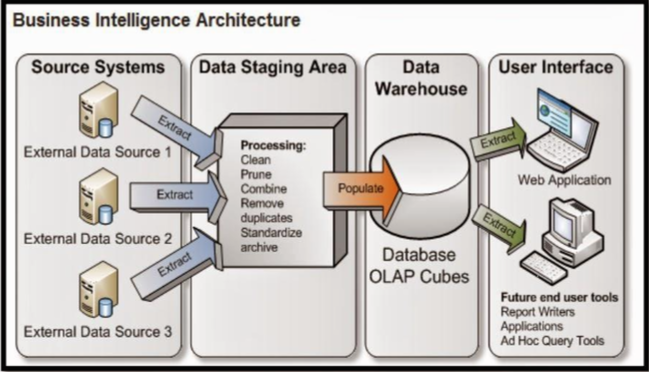
\includegraphics[scale=0.5]{Gambar/arsitektur-kecerdasan-bisnis.png}
	\caption[Arsitektur Kecerdasan Bisnis]{Arsitektur Kecerdasan Bisnis} 
	\label{fig:arsitektur_kecerdasan_bisnis_fig}
\end{figure}

Berdasarkan Gambar \ref{fig:arsitektur_kecerdasan_bisnis_fig} sistem kecerdasan bisnis terdiri dari lima tahap, yaitu:

\begin{enumerate}
	\item \textbf{Source Systems}\\
	\textit{Source systems} merupakan sumber data yang akan disimpan dan dimanfaatkan di sistem kecerdasaan bisnis. Data yang menjadi masukan sangat bermacam-macam. Data dapat berupa data terstruktur seperti basis data relasional, data excel, dan lain-lain. Data juga dapat berupa data yang tidak terstruktur seperti file teks, pesan dari sosial media, gambar, video dan lain-lain.
	
	\item \textbf{Data Staging Area}\\
	Data yang didapat dari berbagai sumber dengan format dan bentuk yang berbagai macam mengakibatkan perlunya pra pengolahan data terlebih dahulu agar mendapatkan data yang sesuai dan siap dimasukan ke dalam \textit{data warehouse}. Pra pengolahan data ini dilakukan di tempat penampungan data sementara yang biasanya disebut \textit{staging area}. Proses pra pengolahan data di \textit{staging area} terdiri dari ETCL (\textit{Extract Trasnform Cleaning and Load}).
		\begin{itemize}
			\item \textit{Extract} adalah proses pemilihan data-data yang dirasa perlu untuk diolah dan dianalisis. Proses \textit{Extract} ini diperlukan karena sumber data yang digunakan dapat sangat banyak dan besar namun tidak seluruh data tersebut dapat dimanfaatkan, sehingga diperlukan pemilihan data-data yang diperlukan saja agar dapat bermanfaat dan menghemat waktu pemrosesan.
			\item \textit{Transform} adalah proses mengubah bentuk data yang sudah ada ke dalam bentuk yang standar sesuai dengan kebutuhan di \textit{data warehouse}. Proses \textit{transform} ini diperlukan karena data yang diambil dari berbagai sumber kemungkinan memiliki standarisasi yang berbeda pula.
			\item \textit{Cleaning} adalah proses pembersihan data-data yang didapat agar hasil keluaran dari sistem kecerdasan bisnis yang dibuat dapat lebih baik kualitasnya.
			\item \textit{Load} adalah proses mengirimkan data-data hasil pembersihan ke dalam \textit{data warehouse}.
		\end{itemize}
	
	\item \textbf{\textit{Data Warehouse}}\\
	\textit{Data warehouse} merupakan basis data yang dirancang untuk kueri dan analisis yang lebih baik dan cepat. \textit{Data warehouse} biasanya mengandung sejarah data transaksi dan mungkin juga data dari sumber lain. Data warehouse memisahkan beban kerja analisis dari beban kerja transaksi dan memungkinkan organisasi untuk menggabungkan / konsolidasi data dari berbagai sumber.
	
	\item \textbf{Analysis \& Reporting}\\
	Sistem kecerdasan bisnis dilengkapi dengan \textit{tools-tools} yang mendukung pembuatan laporan dan analisa data.
	
	\item \textbf{\textit{User Interface}}\\
	\textit{User interface} merupakan tampilan yang digunakan pengguna untuk berinteraksi dengan sistem kecerdasan bisnis. Pengguna dapat melakukan analisis sesuai dengan kebutuhannya dan menghasilkan laporan-laporan yang dibutuhkannya dalam berbagai bentuk seperti diagram atau tabel.
\end{enumerate} 

\section{Pentaho Data Integration}
Pentaho Data Integration (PDI) adalah sebuah program dari Pentaho yang memiliki fungsi utama sebagai \textit{Extraction, Transformation dan Loading} (ETL) program. Pada sebuah sistem kecerdasan bisnis PDI dapat digunakan untuk migrasi data, membersihkan data, \textit{loading} dari file ke database atau sebaliknya dalam volume besar. Selain itu PDI juga mendukung proses ETL dari dan ke sistem terdistribusi Hadoop. 

Elemen utama dari PDI adalah Transformation dan Job. Transformation adalah sekumpulan instruksi untuk merubah input menjadi output yang diinginkan. Sedangkan Job adalah kumpulan instruksi untuk menjalankan transformasi. Komponen-komponen yang ada di PDI seperti Spoon, Pan dan Kitchen. Spoon adalah \textit{user interface} untuk membuat Job dan Transformation. Pan adalah \textit{tools} yang berfungsi membaca, merubah dan menulis data. Sedangkan Kitchen adalah program yang mengeksekusi job. 

Dari sisi tampilan PDI sangat \textit{user-friendly} dan mudah untuk digunakan. PDI menyediakan \textit{graphical user interface} dan \textit{drag-drop} komponen yang memudahkan pengguna dalam menggunakan program.

\section{Sosial Media Twitter}
\label{sec:twitter}
Twitter adalah sebuah situs web yang dimiliki dan dioperasikan oleh Twitter Inc.. Twitter menawarkan jaringan sosial mikroblog dengan panjang pesan maksimal hingga 140 karakter, yang biasanya disebut Tweet. Melalui mikroblog Twitter, pengguna dapat memperbarui status terbaru tentang hal yang sedang mereka pikirkan ataupun berpendapat tentang suatu objek atau fenomena tertentu. Pesan yang dibuat pengguna akan tampil secara langsung dan dapat dilihat seluruh dunia melalui website Twitter atau berbagai aplikasi eksternal lainnya. Untuk menghemat karakter pada sebuah tweet biasanya pengguna menuliskan singkatan, bahasa slang atau emoticon dalam mengkomunikasikan pesannya. 

Pengguna Twitter dapat mengelompokan tweetnya dengan menggunakan \textit{hastags} - kata atau frasa yang diawali dengan tanda "\#". Selain itu pengguna juga dapat menunjuk pengguna lainnya dengan menuliskan \textit{username} mereka diawali dengan tanda "@". Setiap tweet yang dibuat dapat dibalas ataupun di tweet ulang (re-tweet) oleh pengguna lainnya.

Twitter menyediakan Streaming API yang memudahkan pengembang aplikasi untuk mendapatkan tweet-tweet yang dibuat pengguna Twitter secara \textit{realtime}. Streaming API yang tersedia memiliki beberapa jenis sesuai dengan kegunaannya, yaitu:

\begin{enumerate}
	\item \textbf{Public Streams}: Untuk melakukan streaming pada data publik secara \textit{realtime}. Cocok untuk digunakan pada pencarian tweet berdasarkan \textit{user} atau topik tertentu dan \textit{data mining}.
	\item \textbf{User Streams}: Untuk melakukan \textit{streaming} pada \textit{single-user}, hasil streaming terdiri dari data-data yang berkaitan dengan kegiatan \textit{single-user}.
	\item	\textbf{Site Streams}: Merupakan versi \textit{multi-user} dari User Streams. Site Streams dimaksudkan untuk server yang harus terhubung ke Twitter atas nama banyak pengguna.
\end{enumerate}

\begin{figure}
\centering
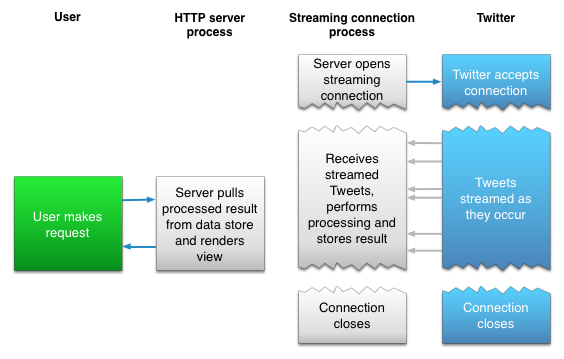
\includegraphics[scale=0.5]{Gambar/streaming-intro-2_1.png}
\caption[Proses Twitter Streaming API]{Proses Twitter Streaming API \cite{TwitterApi:2015}} 
\end{figure}

Twitter Streaming API menggunakan protokol HTTP untuk melakukan \textit{request}. Setiap kali \textit{request} dilakukan sama artinya dengan melakukan koneksi HTTP yang sangat panjang dan melakukan \textit{parsing} terhadap \textit{response} secara bertahap. Koneksi seperti ini dapat dianggap seperti mengunduh file panjang tak terhingga melalui HTTP. Oleh karena itu perlu diperhatikan juga dalam pemilihan \textit{library} yang sesuai, karena banyak \textit{library} yang hanya akan memproses data ketika koneksinya sudah selesai dan hal itu tidak sesuai dengan kondisi di Twitter Streaming API \cite{TwitterApi:2015}.

\section{Sosial Media Instagram}
Instagram adalah sebuah aplikasi berbagi foto yang dapat digunakan oleh pengguna untuk mengambil foto, menerapkan filter digital, dan membagikannya ke teman-teman di yang mengikuti akun instagram. Instagram dapat digunakan dengan mudah oleh para pengguna \textit{smartphone}, oleh karena itu Instagram menjadi salah satu sosial media yang populer saat ini. 

Dalam proses mengunggah foto, pengguna juga dapat memasukan informasi pendukung lainnya seperti lokasi dan keterangan (biasa disebut \textit{caption}). Pada bagian \textit{caption} pengguna dapat menambahkan tag yang diawal dengan tanda \# atau menunjuk pengguna lain yang diawali dengan tanda @. Tag berfungsi sebagai penghubung gambar dengan suatu topik tertentu. 

Instagram menyediakan API untuk digunakan secara umum. Untuk menggunakannya pengembang harus mendaftarkan aplikasinya terlebih dahulu di https://www.instagram.com/developer/. Setelah pengembang mendaftar maka Instagram akan memberikan data-data yang diperlukan untuk melakukan \textit{request} ke API, seperti \textit{client ID, client secret}, website URL, \textit{redirect URL} dan juga \textit{support} email dari aplikasi.

Dengan menggunakan Instagram API, pengembang dapat dengan mudah melakukan autentikasi, mendapatkan data-data pengguna, media, tag, \textit{likes} dan lokasi. \cite{InstagramApi:2016}

\section{AMChart}
AMChart adalah sebuah javascript \textit{library} yang berjalan di sisi \textit{client}. AMChart berfungsi untuk menampilkan grafik-grafik seperti diagram batang, diagram garis, diagram pie ataupun peta interaktif daerah-daerah di seluruh dunia. Contoh-contoh diagram yang dapat dihasilkan oleh AMChart seperti pada Gambar \ref{fig:contoh_amchart}. Penulisan kode program untuk membuat diagram dilakukan menggunakan bahasa Javascript (Listing \ref{lst:contoh_kode_amchart}). 

\begin{figure}
	\centering
	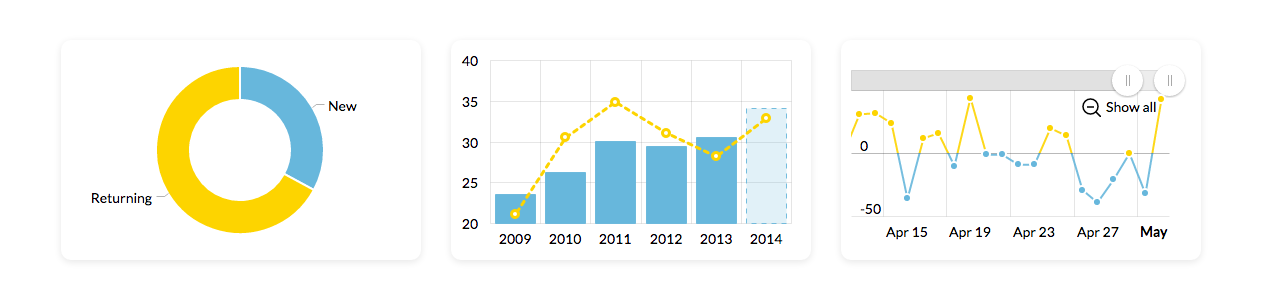
\includegraphics[scale=0.3]{Gambar/contoh-amchart.png}
	\caption[Contoh-contoh diagram AMChart]{Contoh-contoh diagram AMChart\cite{AmCharts:2016}} 
	\label{fig:contoh_amchart}
\end{figure}

\begin{lstlisting}[basicstyle=\tiny,caption=Contoh Kode Diagram Pie di AMChart,label={lst:contoh_kode_amchart}]
var pie_chart = new AmCharts.AmPieChart();
pie_chart.dataProvider = chartData;
pie_chart.titles = [{"text" : "Trend Tipe Lokasi Wisata"}]
pie_chart.titleField = "type";
pie_chart.valueField = "frequencies";
pie_chart.outlineColor = "#FFFFFF";
pie_chart.outlineAlpha = 0.8;
pie_chart.outlineThickness = 2;
pie_chart.creditsPosition = "bottom-right";
pie_chart.write("type");
\end{lstlisting}

\section{Hadoop}
\label{sec:hadoop}

\subsection{Pengertian Hadoop}
\label{sec:pengertian_hadoop}
Apache Hadoop adalah sebuah \textit{framework opensource} yang memungkinkan untuk memproses set data yang besar secara terdistribusi di \textit{cluster} komputer menggunakan model pemrograman yang sederhana. Hadoop dirancang untuk mendeteksi dan menangani kegagalan pada lapisan aplikasi, sehingga memberikan layanan yang \textit{highly-available} pada sekelompok komputer yang masing-masingnya mungkin rentan terhadap kegagalan. Hal tersebut lebih baik dibanding hanya mengandalkan perangkat keras untuk memberikan \textit{high-availability}.

Hadoop bekerja dengan menggunakan penyimpanan terdistribusi dan mentransfer kode program bukan datanya. Hadoop menghindari langkah transmisi yang mahal ketika bekerja dengan kumpulan data besar. Selain itu, redundansi data pada Hadoop memungkinkan Hadoop untuk memulihkan \textit{single node} yang gagal. Membuat program dengan Hadoop akan dimudahkan dengan menggunakan MapReduce \textit{framework}. Yang juga tak kalah penting adalah pengembang tidak perlu khawatir tentang cara melakukan partisi data, menentukan node yang akan melakukan tugas, atau menangani komunikasi antar node. Hadoop sudah menangani ini, sehingga pengembang dapat fokus pada kasusnya.

\subsection{Komponen Utama Hadoop}
\label{sec:komponen_utama_hadoop}
\begin{figure}
	\centering
	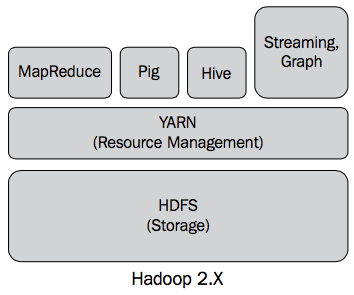
\includegraphics[scale=0.5]{Gambar/hadoop-architecture.png}
	\caption[Arsitektur Komponen Hadoop]{Arsitektur Komponen Hadoop.\cite{holmes2012hadoop}} 
	\label{fig:komponen_utama_hadoop}
\end{figure}

Gambar \ref{fig:komponen_utama_hadoop} menjelas tentang arsitektur Hadoop. Terdapat Hadoop Distributed File System (HDFS), Hadoop Yet Another Resource Negotiator (YARN) dan MapReduce yang menjadi komponen dasar pembentuk Hadoop. Di bagian atasnya terdapat ekosistem lainnya yang dapat berjalan di atas Hadoop.

\subsubsection{Hadoop Distributed File System (HDFS)}
HDFS adalah sebuah file sistem yang didesain untuk memproses data distribusi skala besar di dalam framework seperti MapReduce. HDFS dapat menyimpan sebuat dataset sebesar 100TB sebagai sebuah \textit{single} file.\cite{Lam:2010:HA:1965594} HDFS bisa bersifat \textit{single} node atau \textit{multiple} node. HDFS bukan \textit{native} File System seperti layaknya EXT3, EXT4, FAT atau NTFS. HDFS ada pada layer di atasnya.

HDFS menyimpan suatu data dengan cara membelahnya menjadi potongan-potongan data dengan ukuran tertentu, dan potongan-potongan data ini kemudian disimpan tersebar dalam komputer-komputer yang membentuk \textit{cluster}-nya. Potongan-potongan data tersebut dalam HDFS disebut blok. Ukuran block dapat diatur sesuai kebutuhan 128MB, 256MB ataupun 1GB.

Walaupun data disimpan secara tersebar, dari kacamata pengguna, data tetap terlihat seperti halnya kita mengakses file pada satu komputer. File yang secara fisik disimpan tersebar dalam banyak komputer itu pun dapat diperlakukan layaknya memperlakukan file dalam satu komputer.

Sebagai \textit{distributed file system}, HDFS memiliki komponen-komponen utama berupa NameNode dan DataNode seperti yang digambarkan pada Gambar \ref{fig:hadoop-cluster}. NameNode adalah sebuah komputer yang bertindak sebagai \textit{master}, sedangkan DataNode adalah komputer-komputer dalam Hadoop Cluster yang bertugas sebagai \textit{slaves}. 

NameNode bertanggungjawab menyimpan informasi tentang penempatan blok-blok data dalam Hadoop Cluster. Ia memiliki JobTracker yang bertanggung jawab mengorganisir dan mengontrol blok-blok data yang disimpan tersebar dalam komputer-komputer yang menyusun Hadoop Cluster. Sedangkan DataNode dilengkapi dengan TaskTracker bertugas menyimpan blok-blok data yang dialamatkan kepadanya, dan secara berkala melaporkan kondisinya kepada NameNode. Laporan berkala DataNode kepada NameNode ini disebut Heartbeat. Berdasarkan Heartbeat ini NameNode dapat mengetahui dan menguasai kondisi cluster secara keseluruhan. Sebagai balasan atas Heartbeat dari DataNode, NameNode akan mengirimkan perintah kepada DataNode. 

Secondary NameNode bertugas untuk menyimpan informasi penyimpanan data dan pengolahan data yang ada di NameNode. Fungsinya adalah jika NameNode mati dan diganti dengan NameNode baru maka NameNode baru bisa langsung bekerja dengan mengambil data dari Secondary NameNode. Perlu diingat bahwa Secondary NameNode bukan \textit{backup} jika NameNode mati maka Secondary NameNode otomatis menggantikan.

Jadi, dalam HDFS, NameNode adalah bos yang mengatur dan mengendalikan Hadoop Cluster. Sedangkan, DataNode adalah pekerja yang bertugas menyimpan data dan melaksanakan perintah dari NameNode.

\begin{figure}
	\centering
	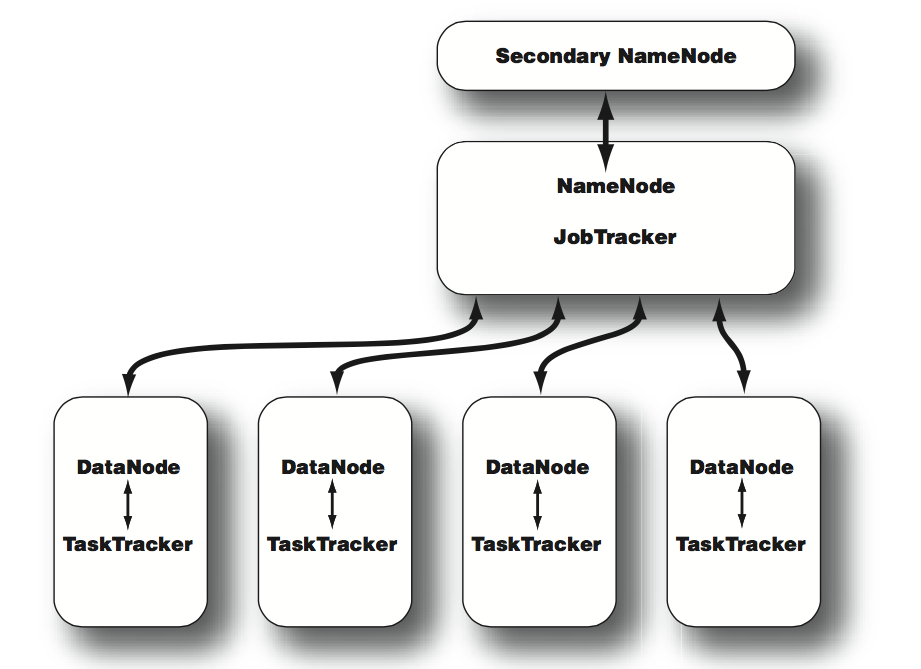
\includegraphics[scale=0.3]{Gambar/hadoop-cluster.png}
	\caption[Hadoop Cluster]{Hadoop Cluster.\cite{Lam:2010:HA:1965594}}
	\label{fig:hadoop-cluster}
\end{figure}
	
\subsubsection{Hadoop MapReduce}
\label{sec:hadoop_mapreduce}
MapReduce adalah sebuah model pemrosesan data\cite{Lam:2010:HA:1965594}. MapReduce ditujukan untuk memproses data berukuran raksasa secara terdistribusi dan paralel dalam \textit{cluster} yang terdiri atas banyak komputer. Dalam memproses data, secara garis besar MapReduce dapat dibagi dalam dua proses yaitu proses \textit{Map} dan proses \textit{Reduce}. Kedua jenis proses ini didistribusikan ke setiap komputer node dalam suatu \textit{cluster} (kelompok komputer yang saling terhubung) dan berjalan secara paralel tanpa saling bergantung satu dengan yang lainnya. Proses \textit{Map} bertugas untuk mengumpulkan informasi dari potongan-potongan data yang terdistribusi dalam tiap komputer dalam \textit{cluster}. Hasilnya diserahkan kepada proses \textit{Reduce} untuk diproses lebih lanjut. Hasil proses Reduce merupakan hasil akhir yang dikirim ke pengguna. \cite{Dean:2008:MSD:1327452.1327492}

MapReduce menggunakan tipe data \textit{list} dan \textit{(key/value) pairs} sebagai data primitif utamanya. \textit{Keys} dan \textit{values} biasanya berupa \textit{integer} atau \textit{string} tapi bisa juga menggunakan \textit{dummy value} atau objek data lainnya. Oleh karena itu fungsi \textit{map} dan \textit{reduce} harus bisa menangani berbagai data tersebut.

Di dalam \textit{framework} MapReduce, aplikasi ditulis dengan memspesifikasikan \textit{mapper} dan \textit{reducer}. Berikut adalah contoh lengkap aliran data yang terjadi pada MapReduce.

\begin{table}[H]
	\centering
	\begin{tabular}{| l | c | c |}
		\hline
		 & Input & Output \\
	 	\hline
		map & <k1, v1> & list(<k2, v2>) \\
		reduce & <k3, list(v2)> & list(<k3, v3>) \\ 
		\hline
	\end{tabular}	
	\caption{Input dan Output pada MapReduce} \label{tab:mapreduce_process}
\end{table}	

\begin{enumerate}
	\item Masukan data ke dalam aplikasi harus terstruktur dalam bentuk \textit{lists} dari \textit{(key/value) pairs}, list(<k1, v1>). Dalam pengaplikasiannya input dapat dibuat seperti contoh berikut, list(<String filename, String filecontent>) atau list(<Integer messageid, String message>).
	\item Setelah masukan diterima maka proses mapper akan dijalankan. Proses mapper akan membagi masukan \textit{lists} dari \textit{(key/value) pairs} menjadi masing-masing \textit{(key/value) pairs}, <k1, v1>. \textit{Mapper} mengubah setiap <k1, v1> dan memasangkannya menjadi list(<k2, v2>) secara acak. Pada contoh kasus penghitung kata, mapper mendapatkan masukan berupa list(<String filename, String filecontent>), kemudian \textit{list} dipecah menjadi <String filename, String filecontent> \textit{pairs}. Teks yang terdapat pada filecontent dihitung satu per satu yang akan menghasilkan keluaran berupa <String word, Integer count>, contoh: <"hello", 1>, <"hello", 2>, <"world", 1>. 
	\item Seluruh keluaran yang dihasilkan dari proses Mapper dikumpulkan dan menjadi sebuah \textit{list of <k2, v2> pairs} raksasa. Semua pasangan yang memiliki nilai k2 yang sama akan dikelompokan menjadi satu pasangan baru yaitu <k2, list(v2)>. Kemudian \textit{framework} akan menjalakan fungsi \textit{reducer} untuk memproses masing-masing pasangan baru menjadi list(<k3, v3>). Pada contoh kasus penghitung kata, misal ada pasangan <"hello", 1> sebanyak dua buah, maka reducer akan memprosesnya menjadi <"hello", list(1,1)> dan keluaran yang dihasilkan oleh reducer akan menjadi <"hello", 2>. Hasil dari masing-masing pasangan akan disatukan kembali dalam bentuk list, misal list(<"hello", 2>, <"world", 1>).
\end{enumerate} 

Gambar \ref{fig:mapper_works} menggambarkan cara kerja Map pada HDFS. 
\begin{enumerate}
	\item Masukan data berukuran besar dari pesan, log, sensor, dsb ke dalam HDFS yang dibagi ke dalam beberapa block data, kemudian dibagi ke dalam \textit{record-record}.
	\item Data yang sudah dibagi-bagi ke DataNode melakukan tugas Map. 
	\item Keluaran yang dihasilkan diurutkan dan akan menjadi masukan bagi reducer.
\end{enumerate}


\begin{figure}
	\centering
	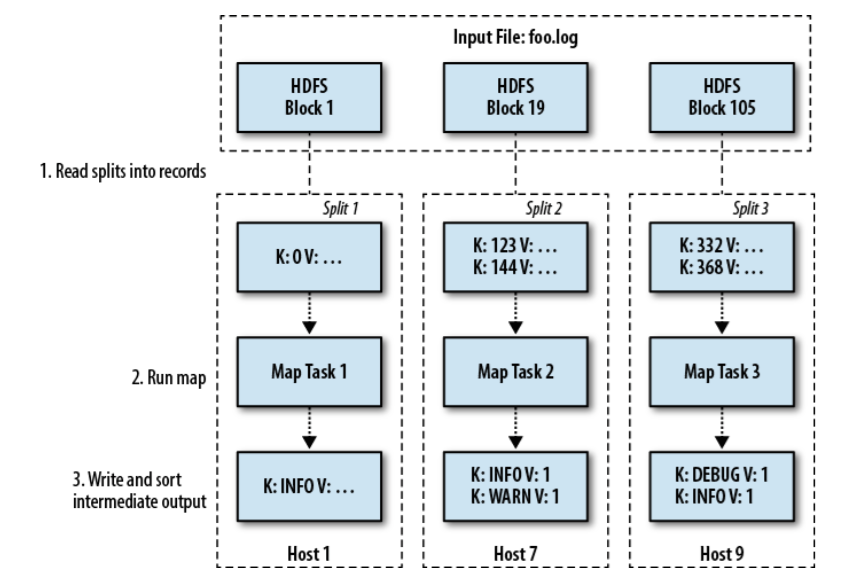
\includegraphics[scale=0.5]{Gambar/how-mapper-works.png}
	\caption[Cara  Kerja Map]{Cara Kerja Map.\cite{sammer2012hadoop}}
	\label{fig:mapper_works}
\end{figure}

Gambar \ref{fig:reducer_works} menggambarkan cara kerja Reduce pada HDFS.
\begin{enumerate}
	\item Masukan data dari hasil fungsi mapper.
	\item Menjalankan fungsi reduce untuk menyatukan data kembali.
	\item Keluaran yang dihasilkan disimpan kembali ke dalam HDFS.
\end{enumerate}

\begin{figure}
	\centering
	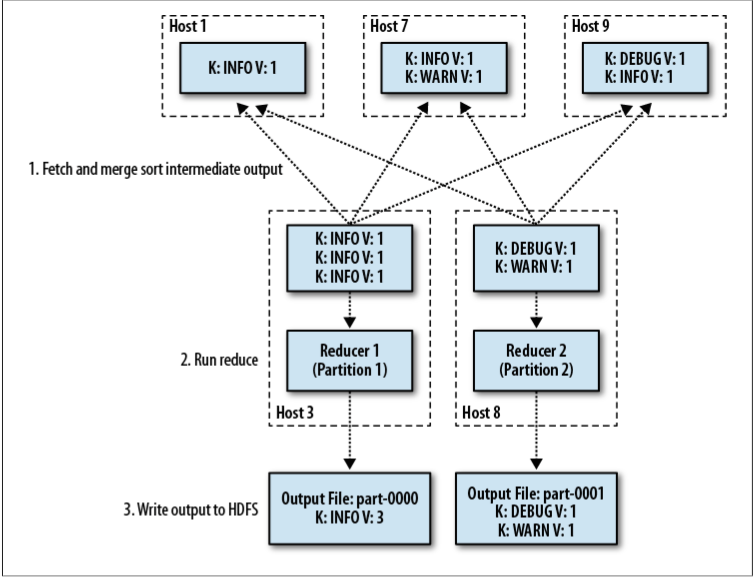
\includegraphics[scale=0.5]{Gambar/how-reducer-works.png}
	\caption[Cara  Kerja Reduce]{Cara Kerja Reduce.\cite{sammer2012hadoop}}
	\label{fig:reducer_works}
\end{figure}
	
\subsubsection{Hadoop Hadoop Yet Another Resource Negotiator (YARN)}
Hadoop Yet Another Resource Negotiator atau YARN adalah teknologi untuk mengatur \textit{resource} dan \textit{scheduling} pada sebuah cluster. YARN berada suatu layer diatas HDFS yang memungkinkan aplikasi lain untuk memproses data yang sama di Hadoop secara paralel dengan MapReduce. Pada Hadoop versi 2.x MapReduce dianggap sebuah aplikasi YARN.

\subsection{Hive}
\label{sec:hive}
Apache Hive adalah perangkat lunak \textit{data warehouse} yang memfasilitasi kueri dan mengelola dataset besar yang berada dalam penyimpanan terdistribusikan. Apache Hive dibangun dan berjalan di atas Apache Hadoop. Pada awalnya Hive dibuat oleh Facebook untuk memproses data \textit{user} dan log yang sangat besar. Saat ini Hive sudah menjadi proyek \textit{open source} dengan banyak kontributor dan merupakan subproyek dari Hadoop.  

Target dari pengguna Hive adalah para data analis yang terbiasa menggunakan SQL dalam pekerjaannya. Hive mendefinisikan sebuah SQL sederhana seperti bahasa kueri yang disebut HiveQL. HiveQL memungkingkan pengguna yang terbiasa dengan SQL untuk melakukan kueri pada data. Dengan menggunakan Hive para pengguna dapat melakukan kueri-kueri untuk \textit{summarization} dan data analisis pada lingkungan data Hadoop. 

HiveQL terinspirasi untuk memisahkan bahasa yang digunakan pengguna dengan kompleksitas MapReduce. HiveQL menggunakan kembali konsep dari \textit{database} relasional, seperti tabel, baris, kolom, dan skema, untuk memudahkan pembelajaran. Namun perlu diingat karena Hive dibangun di atas Hadoop dan sifatnya yang dirancang untuk tipe \textit{batch oriented} dalam pemrosesan datanya, maka Hive bukanlah pengganti langsung untuk \textit{data warehouse} SQL tradisional.

Hive memiliki sedikit perbedaan dengan Hadoop dalam penyimpanan datanya. Di Hadoop data disimpan dalam bentuk \textit{flat file}, sedangkan di Hive data dapat menggunakan direktori untuk melakukan partisi data. Dengan adanya partisi pada data di Hive, maka proses pencarian dapat dilakukan dengan lebih baik daripada disimpan dalam bentuk \textit{flat file}. Untuk mendukung fitur-fitur tambahan ini, Hive memerlukan komponen tambahan seperti metastore. Metastore berfungsi untuk menyimpan informasi skema. Metastore ini biasanya berada dalam basis data relasional. Metastore disimpan di dalam sebuah direktori di dalam Hive.

Pengguna dapat berinteraksi dengan Hive menggunakan beberapa metode, termasuk GUI Web dan Java Database Connectivity (JDBC). Gambar \ref{fig:hive_architecture} menggambarkan arsitektur dari Hive. Pada arsitektur Hive terdapat beberapa macam \textit{client driver} (Thrift, JDBC dan ODBC) yang dapat digunakan untuk menjembatani \textit{client} dengan \textit{service}. Metastore merupakan komponen penting yang membantu menentukan bagaimana kueri akan dijalankan oleh Hive.

\begin{figure}
	\centering
	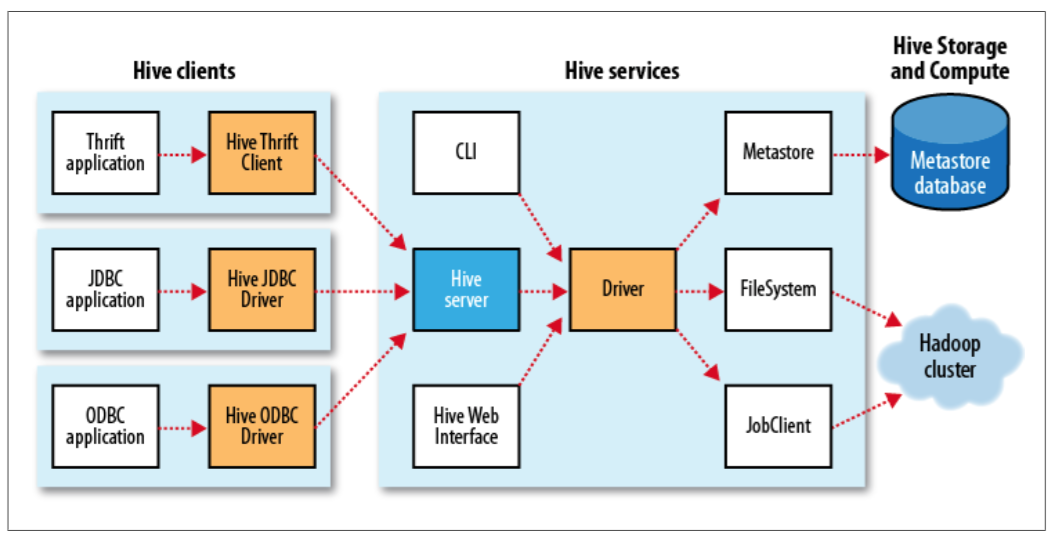
\includegraphics[scale=0.4]{Gambar/arsitektur-hive.png}
	\caption[Arsitektur Hive]{Arsitektur Hive\cite{white2012hadoop}} 
	\label{fig:hive_architecture}
\end{figure}

Hive mendukung tipe data primitif dan tipe data yang kompleks. Tipe data primitif terdiri dari TinyInt, SmallInt, Int, BigInt, Float, Double, Boolean, String, Binary, dan Timestamp sedangkan untuk tipe data yang kompleks terdiri dari Array, Map, Struct.

\subsubsection{\textit{Managed Tables} dan \textit{External Tables}}
Ketika tabel dibuat, Hive menerapkan \textit{managed table} yang akan memindahkan data ke dalam direktori \textit{warehouse} di dalam HDFS. Alternatif lainnya, dapat menggunakan \textit{external table} agar tabel yang dibuat dapat disimpan di luar direktori \textit{warehouse} namun masih di dalam HDFS. 

Pada prinsipnya kedua jenis tabel ini hampir mirip, yang membedakan hanyalah ketika proses \textit{drop table}. \textit{Managed table} ketika menjalankan kueri \textit{drop table} maka akan melakukan penghapusan metadata serta file data di direktori \textit{warehouse}. Sedangkan \textit{external table} ketika menjalankan kueri \textit{drop table} maka akan melakukan penghapusan metadatanya saja sehingga file data di luar direktori \textit{warehouse} tetap utuh.

\subsubsection{DDL Operation Hive}
Seperti layaknya sebuah SQL tradisional, Hive memiliki fungsi-fungsi \textit{Data Definition Language} (DDL) yang dapat digunakan untuk membantu pengguna dalam membuat dan mengelola tabel-tabel, view, index ataupun function. Berikut adalah \textit{statement} DDL yang dapat digunakan oleh pengguna.

\begin{itemize}
	\item CREATE DATABASE/SCHEMA, TABLE, VIEW, FUNCTION, INDEX
	\item DROP DATABASE/SCHEMA, TABLE, VIEW, INDEX
	\item TRUNCATE TABLE
	\item ALTER DATABASE/SCHEMA, TABLE, VIEW
	\item MSCK REPAIR TABLE (or ALTER TABLE RECOVER PARTITIONS)
	\item SHOW DATABASES/SCHEMAS, TABLES, TBLPROPERTIES, PARTITIONS, FUNCTIONS, INDEX, COLUMNS, CREATE TABLE
	\item DESCRIBE DATABASE SCHEMA
\end{itemize}

Berikut adalah format-format dan contoh-contoh DDL pada Hive.

\begin{lstlisting}[language=sql,basicstyle=\tiny,caption=DDL untuk create database]
CREATE (DATABASE|SCHEMA) [IF NOT EXISTS] database_name
  [COMMENT database_comment]
  [LOCATION hdfs_path]
  [WITH DBPROPERTIES (property_name=property_value, ...)];
\end{lstlisting}

\begin{lstlisting}[language=sql,basicstyle=\tiny,caption=DDL untuk drop database]
DROP (DATABASE|SCHEMA) [IF EXISTS] database_name [RESTRICT|CASCADE];
\end{lstlisting}

\begin{lstlisting}[language=sql,basicstyle=\tiny,caption=DDL untuk alter database]
ALTER (DATABASE|SCHEMA) database_name SET DBPROPERTIES (property_name=property_value, ...);   -- (Note: SCHEMA added in Hive 0.14.0)
ALTER (DATABASE|SCHEMA) database_name SET OWNER [USER|ROLE] user_or_role;   -- (Note: Hive 0.13.0 and later; SCHEMA added in Hive 0.14.0)
\end{lstlisting}

\begin{lstlisting}[language=sql,basicstyle=\tiny,caption=DDL untuk use database]
USE database_name;
USE DEFAULT;
\end{lstlisting}

\begin{lstlisting}[language=sql,basicstyle=\tiny,caption=Contoh DDL untuk membuat tabel dengan partisi]
create table table_name (
  id			int,
  dtDontQuery	string,
  name			string
)
partitioned by (date string)
\end{lstlisting}

\begin{lstlisting}[language=sql,basicstyle=\tiny,caption=Contoh DDL untuk drop tabel]
DROP TABLE [IF EXISTS] table_name [PURGE];     -- (Note: PURGE available in Hive 0.14.0 and later)
\end{lstlisting}

\subsubsection{DML Operation Hive}
Data Manipulation Languange (DML) digunakan untuk melakukan kueri-kueri terhadap isi data dari suatu tabel. Pada Hive ada beberapa operasi dalam melakukan manipulasi data seperti \textit{load, insert, update}, dan \textit{delete}. 

\textbf{Load}\\
Pada proses \textit{load} Hive tidak melakukan transformasi data apapun. Proses ini murni hanya untuk melakukan operasi \textit{copy/move} data file ke dalam lokasi yang sesuai pada tabel Hive. Berikut \textit{syntax} dari proses \textit{load} pada Hive.

\begin{lstlisting}[language=sql,basicstyle=\tiny,caption=Syntax DML Load]
LOAD DATA [LOCAL] INPATH 'filepath' [OVERWRITE] INTO TABLE tablename [PARTITION (partcol1=val1, partcol2=val2 ...)]
\end{lstlisting}

\begin{lstlisting}[language=sql,basicstyle=\tiny,caption=Contoh DML Load]
LOAD DATA INPATH '/user/myname/kv2.txt' OVERWRITE INTO TABLE invites PARTITION (ds='2008-08-15');
\end{lstlisting}

\textbf{Penjelasan: }
\begin{itemize}
	\item \textit{filepath} dapat berupa:
		\begin{itemize}
			\item sebuah \textit{relative path}, seperti project/data1
			\item sebuah \textit{absolut path}, seperti /user/hive/project/data1
			\item sebuah \textit{full URI}, seperti hdfs://namenode:9000/user/hive/project/data1
		\end{itemize}
	\item Target yang dimasukan dapat berupa tabel atau partisi. Jika tabel dipartisi, maka harus menentukan partisi tertentu dari tabel yang akan dimuat berupa nilai dari seluruh kolom yang dipartisi.
	\item Keyword LOCAL sifatnya adalah optional, jika digunakan maka yang akan terjadi adalah perintah load akan melihat \textit{filepath} di the local file system. Namun jika keyword LOCAL tidak digunakan maka yang akan terjadi adalah Hive akan menggunakan URI \textit{filepath} lengkap.
\end{itemize}

Beberapa catatan yang perlu diingat dalam menggunakan kueri load ini adalah
\begin{itemize}
	\item \textit{filepath} tidak boleh terdiri dari sub direktori
	\item Jika \textit{keyword} LOCAL tidak digunakan, \textit{filepath} harus mengacu ke file dalam \textit{filesystem} yang sama dengan tabel atau partisi.
\end{itemize}

\textbf{Insert}\\
Perintah \textit{insert} berfungsi untuk memasukan data ke dalam tabel pada Hive. \textit{Syntax} kueri insert pada Hive memiliki \textit{standard syntax, multiple insert dan dynamic partition insert}. \textit{Standard syntax} merupakan kueri dasar dari \textit{insert} dalam melakukan input data ke dalam sebuah tabel. \textit{Multiple insert} digunakan untuk melakukan proses input data ke dalam beberapa tabel sekaligus. Sedangkan \textit{dynamic partition insert} digunakan untuk melakukan input data menggunakan partisi.

\begin{lstlisting}[language=sql,basicstyle=\tiny,caption=Syntax DML Insert]
Standard syntax:
INSERT OVERWRITE TABLE tablename1 [PARTITION (partcol1=val1, partcol2=val2 ...) [IF NOT EXISTS]] select_statement1 FROM from_statement;
INSERT INTO TABLE tablename1 [PARTITION (partcol1=val1, partcol2=val2 ...)] select_statement1 FROM from_statement;
 
Hive extension (multiple inserts):
FROM from_statement
INSERT OVERWRITE TABLE tablename1 [PARTITION (partcol1=val1, partcol2=val2 ...) [IF NOT EXISTS]] select_statement1
[INSERT OVERWRITE TABLE tablename2 [PARTITION ... [IF NOT EXISTS]] select_statement2]
[INSERT INTO TABLE tablename2 [PARTITION ...] select_statement2] ...;
FROM from_statement
INSERT INTO TABLE tablename1 [PARTITION (partcol1=val1, partcol2=val2 ...)] select_statement1
[INSERT INTO TABLE tablename2 [PARTITION ...] select_statement2]
[INSERT OVERWRITE TABLE tablename2 [PARTITION ... [IF NOT EXISTS]] select_statement2] ...;
 
Hive extension (dynamic partition inserts):
INSERT OVERWRITE TABLE tablename PARTITION (partcol1[=val1], partcol2[=val2] ...) select_statement FROM from_statement;
INSERT INTO TABLE tablename PARTITION (partcol1[=val1], partcol2[=val2] ...) select_statement FROM from_statement;
\end{lstlisting}

\begin{lstlisting}[language=sql,basicstyle=\tiny,caption=Contoh DML Insert]
INSERT OVERWRITE TABLE events SELECT a.* FROM profiles a;
INSERT OVERWRITE TABLE events SELECT a.* FROM profiles a WHERE a.key < 100;
INSERT OVERWRITE LOCAL DIRECTORY '/tmp/reg_3' SELECT a.* FROM events a;
INSERT OVERWRITE DIRECTORY '/tmp/reg_4' select a.invites, a.pokes FROM profiles a;
INSERT OVERWRITE DIRECTORY '/tmp/reg_5' SELECT COUNT(*) FROM invites a WHERE a.ds='2008-08-15';
INSERT OVERWRITE DIRECTORY '/tmp/reg_5' SELECT a.foo, a.bar FROM invites a;
INSERT OVERWRITE LOCAL DIRECTORY '/tmp/sum' SELECT SUM(a.pc) FROM pc1 a;
FROM invites a INSERT OVERWRITE TABLE events SELECT a.bar, count(*) WHERE a.foo > 0 GROUP BY a.bar;
FROM pokes t1 JOIN invites t2 ON (t1.bar = t2.bar) INSERT OVERWRITE TABLE events SELECT t1.bar, t1.foo, t2.foo;

//Multitable insert
FROM src
INSERT OVERWRITE TABLE dest1 SELECT src.* WHERE src.key < 100
INSERT OVERWRITE TABLE dest2 SELECT src.key, src.value WHERE src.key >= 100 and src.key < 200
INSERT OVERWRITE TABLE dest3 PARTITION(ds='2008-04-08', hr='12') SELECT src.key WHERE src.key >= 200 and src.key < 300
INSERT OVERWRITE LOCAL DIRECTORY '/tmp/dest4.out' SELECT src.value WHERE src.key >= 300;
\end{lstlisting}


\textbf{Update}\\
Perintah \textit{update} berfungsi untuk melakukan perubahan data yang sudah ada pada tabel. Perintah \textit{update} pada Hive cukup sederhana layaknya pada SQL \textit{syntax} lainnya. 

\begin{lstlisting}[language=sql,basicstyle=\tiny,caption=Syntax DML Update]
UPDATE tablename SET column = value [, column = value ...] [WHERE expression]
\end{lstlisting}

\textbf{Penjelasan:}
\begin{itemize}
	\item \textit{Value} yang diberikan harus sebuah ekspresi yang dapat dilakukan oleh Hive. Sehingga operator aritmatika, cast, literal dll dapat digunakan. Tetapi nilai dari sub kueri tidak dapat digunakan dalam pemberian \textit{value}.
	\item Kolom yang dipartisi tidak dapat diperbaharui dengan perintah update.
\end{itemize}

\textbf{Delete}\\
Perintah \textit{delete} berfungsi untuk melakukan penghapusan data yang sudah ada pada tabel. Perintah \textit{delete} pada Hive cukup sederhana layaknya pada SQL \textit{syntax} lainnya. 

\begin{lstlisting}[language=sql,basicstyle=\tiny,caption=Syntax DML Delete]
DELETE FROM tablename [WHERE expression]
\end{lstlisting}

\subsubsection{SQL Operation Hive}
Operation SQL adalah operasi yang dapat digunakan untuk memperoleh data atau isi dari suatu tabel. Berikut adalah contoh-contoh dari syntax SQL operation pada Hive.

\begin{lstlisting}[language=sql,basicstyle=\tiny,caption=Syntax DML SQL Operation]
//Basic select dengan kriteria 
SELECT page_views.*
FROM page_views
WHERE page_views.date >= '2008-03-01' AND page_views.date <= '2008-03-31'

//Perintah select dengan sub kueri dan grouping
SELECT col1 FROM (SELECT col1, SUM(col2) AS col2sum FROM t1 GROUP BY col1) t2 WHERE t2.col2sum > 10

//Perintah select yang ditampilkan berurut menaik dengan limit 5 buah record
SELECT * FROM sales SORT BY amount DESC LIMIT 5

//Perintah select dengan regex dalam pemilihan kolom-kolomnya
SELECT `(ds|hr)?+.+` FROM sales

//Perintah select dengan join
SELECT a.* FROM a JOIN b ON (a.id = b.id AND a.department = b.department)

//Perintah select dengan union
SELECT key FROM (SELECT key FROM src ORDER BY key LIMIT 10)subq1
UNION
SELECT key FROM (SELECT key FROM src1 ORDER BY key LIMIT 10)subq2
\end{lstlisting}
	
\subsection{Sqoop}
\label{sec:sqoop}
Salah satu kekuatan Hadoop adalah kemampuannya untuk bekerja dengan berbagai bentuk data. Seluruh data-data yang tersimpan di dalam HDFS dapat langsung dimanfaatkan dan dijalankan oleh program MapReduce untuk mendapatkan informasi yang berharga. Namun untuk berinteraksi dengan tempat penyimpan data lainnya di luar HDFS, program MapReduce membutuhkan bantuan Application Program Interface (API) eksternal untuk mendapatkan datanya. Salah satu tempat penyimpanan data yang sering digunakan adalah basis data relasional (RDBMS).

Apache Sqoop adalah salah satu \textit{tool open source} yang memungkinkan pengguna untuk mengekstrak data dari tempat penyimpanan data lainnya untuk kemudian disimpan di dalam HDFS. Data yang dapat diimpor oleh Sqoop adalah data yang sifatnya terstruktur seperti basis data relasional (RDBMS). Selain mengekstrak data dari luar HDFS, Sqoop juga dapat melakukan ekspor data dari dalam HDFS ke tempat penyimpanan data lainnya.

\subsubsection{Konektor Sqoop}
\label{sec:konektor_sqoop}
Sqoop adalah sebuah ekstensi yang dapat digunakan untuk melakukan ekspor dan impor data dari dan ke HDFS. Sqoop membutuhkan konektor dalam melakukan proses ekspor maupun impor data. Sqoop pada dasarnya sudah dilengkapi dengan konektor-konektor untuk basis data relasional yang populer seperti MySQL, PostgreSQL, Oracle, SQL Server dan DB2. Selain itu Sqoop juga dilengkapi konektor Java Database Connectivity (JDBC), sehingga Sqoop dapat terkoneksi dengan basis data yang  mendukung protokol JDBC. Selain \textit{built-in} konektor pada Sqoop, terdapat juga banyak konektor pihak ke tiga yang dapat melakukan koneksi ke \textit{datawarehouse} \textit{enterprise} seperti Netezza, Teradata, Oracle ataupun ke basis data NoSQL seperti Couchbase. 

\subsubsection{Impor Data Sqoop}
\label{sec:impor_data_sqoop}
Tool impor data Sqoop berfungsi untuk melakukan pemindahan data dari luar HDFS ke dalam HDFS. Tool ini akan berjalan pada sebuah MapReduce yang melakukan koneksi dan membaca basis data di luar HDFS. Pada dasarnya, operasi impor ini akan dilakukan menggunakan empat buah \textit{task} map secara parallel untuk mempercepat proses impor data. Setiap \textit{task}  akan menulis hasilnya ke dalam sebuah file berbeda namun masih di dalam sebuah direktori yang sama. Namun pada kebutuhan tertentu pengguna dapat mengatur jumlah \textit{task} map yang akan digunakan. Sqoop akan membuat file-file teks dengan pemisah koma antar kolomnya. Pemisah dapat dispesifikasikan apabila diperlukan pemisah dengan karakter lainnya. 

\begin{figure}
	\centering
	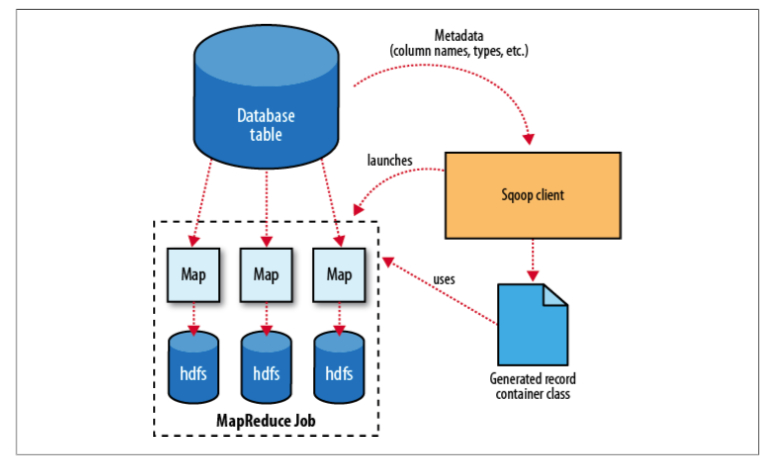
\includegraphics[scale=0.5]{Gambar/sqoop-import.png}
	\caption[Proses Impor Sqoop]{Proses Impor Sqoop \cite{white2012hadoop}} 
	\label{fig:sqoop_import}
\end{figure}

Gambar \ref{fig:sqoop_import} menggambarkan proses kerja impor pada Sqoop. Sqoop client akan membaca Metadata dari basisdata seperti \textit{field}, tipe data, dll melalui konektor JDBC. Kemudian Sqoop client secara otomatis akan membuat sebuah file java yang berisi kelas untuk melakukan proses impor menggunakan MapReduce. 

Berikut adalah contoh-contoh perintah pada Sqoop.

\begin{lstlisting}[caption=Perintah Impor Sqoop dari Basis Data MySQL ke HDFS]
	sqoop import --connect jdbc:mysql://localhost/nama_database \
	--username root  \
	--password your_password  \
	--table nama_tabel 
\end{lstlisting}

Pada kode di atas, Sqoop akan melakukan impor data dari basis data MySQL ke dalam HDFS.

\begin{lstlisting}[caption=Perintah Impor Sqoop dari Basis Data MySQL ke Hive]
	sqoop import --connect jdbc:mysql://localhost/nama_database \
	--table nama_tabel \ 
	--username root  \
	--password your_password \
	--hive-import \
	--fields-terminated-by ','  \
	--lines-terminated-by '\n'
\end{lstlisting}

Pada kode di atas, Sqoop akan melakukan impor data dari basis data MySQL ke dalam Hive dengan karakter koma sebagai pemisah antar \textit{field} dan baris baru sebagai pemisah antar \textit{record}.

\subsubsection{Ekspor Data Sqoop}
\label{sec:ekspor_data_sqoop}
Tool ekspor data Sqoop berfungsi untuk melakukan pemindahan data dari dalam HDFS ke luar HDFS. Cara kerja dari proses ekspor ini sangatlah mirip dengan proses impor yang sudah dibahas sebelumnya. 

(Lihat gambar \ref{fig:sqoop_ekspor}.) Sebelum melakukan ekspor, Sqoop client memulai dengan melakukan koneksi ke basis data menggunakan koneksi \textit{string} (kebanyakan sistem menggunakan JDBC). Kemudian Sqoop client akan membuat sebuah file kelas Java berdasarkan metadata pada tabel yang dituju. File yg dihasilkan dapat melakukan \textit{parsing} terhadap \textit{record-record} pada file teks di HDFS dan memasukan hasilnya ke dalam tabel. Setelah file kelas Java dibuat, maka sebuah MapReduce \textit{job} dimulai dan bertugas untuk membaca file di HDFS, \textit{parsing} data menggunakan kelas Java yang sudah dibuat, dan melakukan strategi expor data ke basisdata yang dituju.

\begin{figure}
	\centering
	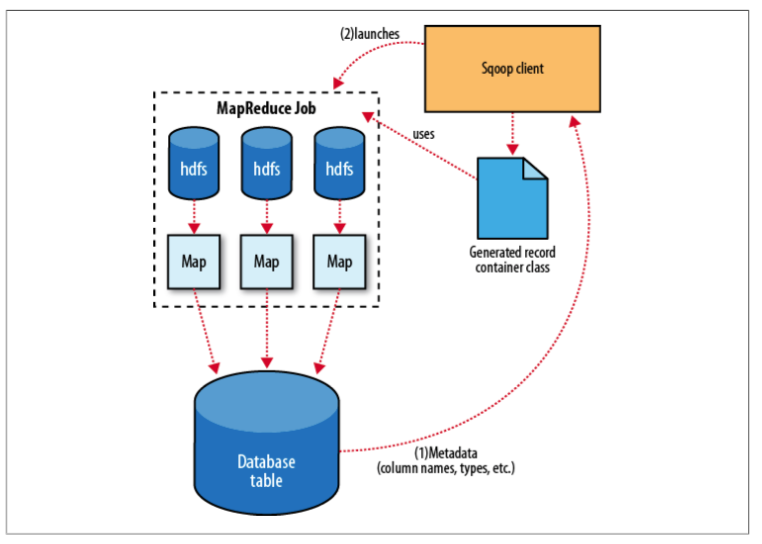
\includegraphics[scale=0.5]{Gambar/sqoop-export.png}
	\caption[Proses Ekspor Sqoop]{Proses Ekspor Sqoop \cite{white2012hadoop}} 
	\label{fig:sqoop_ekspor}
\end{figure}

\begin{lstlisting}[caption=Perintah Ekspor Sqoop dari HDFS ke Basis Data MySQL]
	sqoop export --connect jdbc:mysql://localhost/nama_database \
	--username root \
	--password your_password \
	--table nama_tabel  \
	--export-dir /path/to/your/data
\end{lstlisting}

Pada kode di atas, Sqoop akan melakukan ekspor data dari HDFS ke dalam basis data MySQL.

\begin{lstlisting}[caption=Perintah Ekspor Sqoop dari Hive ke Basis Data MySQL]
	sqoop import --connect jdbc:mysql://localhost/nama_database \
	--table nama_tabel \ 
	--username root \
	--password your_password \
	--export-dir /path/to/your/data \
	--fields-terminated-by ','  \
	--lines-terminated-by '\n'
\end{lstlisting}

Pada kode di atas, Sqoop akan melakukan ekspor data dari Hive ke dalam basis data MySQL dengan karakter koma sebagai pemisah antar \textit{field} dan baris baru sebagai pemisah antar \textit{record}.
